% ============================================================
% FEE3411 Control Systems A -- Lecture notes, Week 01
% Topic: Introduction and control system components
%
% Build:  latexmk -pdf week-01-notes.tex
% Needs:  ../tex/preamble.tex (this file lives in Notes/).
% ============================================================
\documentclass[11pt,a4paper]{article}
\usepackage[margin=25mm]{geometry}
% ============================================================
% FEE3411 Control Systems A -- shared preamble
% Used by both the lecture notes (article) and the slides (beamer).
% ============================================================
\usepackage[T1]{fontenc}
% lmodern gives cleaner PDF fonts but is absent from minimal TeX installs.
% Load it only if present, so this preamble builds anywhere.
\IfFileExists{lmodern.sty}{\usepackage{lmodern}}{}
\usepackage{amsmath,amssymb,amsthm}
\usepackage{graphicx}
\usepackage{booktabs}
\usepackage{siunitx}
\usepackage{tikz}
\usepackage{circuitikz}
\usepackage{pgfplots}
\pgfplotsset{compat=1.18}
\usetikzlibrary{arrows.meta,positioning,calc,decorations.markings,shapes.geometric}
\usepackage[most]{tcolorbox}
\usepackage{xcolor}

% ---- Course colours -------------------------------------------------
\definecolor{fnavy}{HTML}{1F3864}
\definecolor{faccent}{HTML}{2E5E4E}
\definecolor{fflag}{HTML}{9C4221}

% ---- Block-diagram style --------------------------------------------
\tikzset{
  block/.style   = {draw, thick, rectangle, minimum height=2.6em,
                    minimum width=3.2em, align=center},
  sumnode/.style = {draw, thick, circle, inner sep=0pt, minimum size=1.6em},
  pickoff/.style = {fill, circle, inner sep=0pt, minimum size=3pt},
  sig/.style     = {-{Latex[length=2mm]}, thick},
}

% ---- Summing-junction signs -----------------------------------------
% \sumsign{<node>}{<angle>}{<+ or ->} places a sign just outside the circle.
\newcommand{\sumsign}[3]{\node[font=\small] at ($(#1)+(#2:0.5)$) {$#3$};}

% ---- Boxed environments ---------------------------------------------
\newtcolorbox{keyidea}[1][]{colback=fnavy!5,colframe=fnavy,
  fonttitle=\bfseries,title=Key idea,#1}
\newtcolorbox{workedex}[1][]{colback=faccent!5,colframe=faccent,
  fonttitle=\bfseries,title=Worked example,#1}
\newtcolorbox{pitfall}[1][]{colback=fflag!5,colframe=fflag,
  fonttitle=\bfseries,title=Common pitfall,#1}

% ---- Shorthands ------------------------------------------------------
\newcommand{\Lap}{\mathcal{L}}
\newcommand{\jw}{\mathrm{j}\omega}
\newcommand{\wn}{\omega_{n}}
\newcommand{\zt}{\zeta}
\newcommand{\TF}[1]{#1(s)}

% ---- Week title machinery -------------------------------------------
\usepackage{fancyhdr}
\newcommand{\thecoursecode}{FEE3411}
\newcommand{\thecoursename}{Control Systems A}
\newcommand{\wknum}{}
\newcommand{\wktopic}{}
\newcommand{\weeknumber}[1]{\renewcommand{\wknum}{#1}}
\newcommand{\weektopic}[1]{\renewcommand{\wktopic}{#1}}
\newcommand{\weektitle}{%
  \thispagestyle{plain}%
  \begin{center}
    {\large\sffamily\bfseries\color{fnavy}\thecoursecode: \thecoursename}\\[2pt]
    {\Huge\sffamily\bfseries Week \wknum}\\[4pt]
    {\LARGE\sffamily\color{fnavy}\wktopic}\\[6pt]
    \rule{\textwidth}{1.2pt}
  \end{center}\vspace{4pt}%
  \pagestyle{fancy}\fancyhf{}%
  \fancyhead[L]{\footnotesize\color{gray}\thecoursecode\ Week \wknum\ --- \wktopic}%
  \fancyhead[R]{\footnotesize\color{gray}\thepage}%
  \renewcommand{\headrulewidth}{0.4pt}%
}

% ---- Outcomes and reading boxes -------------------------------------
\newenvironment{outcomes}
  {\begin{tcolorbox}[colback=white,colframe=fnavy!60,
      fonttitle=\bfseries,title=By the end of this week you should be able to]
   \begin{itemize}[leftmargin=*]}
  {\end{itemize}\end{tcolorbox}}

\newtcolorbox{readingbox}{colback=gray!5,colframe=gray!50,
  fonttitle=\bfseries,title=Reading}

% enumitem must NOT be loaded under beamer: it overwrites beamer's itemize
% templates and the bullet markers silently disappear. The notes (article) get
% it; the slides (beamer) use beamer's own list machinery instead.
\makeatletter
\@ifclassloaded{beamer}{}{\usepackage{enumitem}}
\makeatother


\weeknumber{1}
\weektopic{Introduction and Control System Components}

\begin{document}
\weektitle

% --------------------------------------------------------------------
\section*{What this week covers}

\begin{outcomes}
\item Name the six parts of a feedback control system --- plant, actuator,
      sensor, controller, reference and disturbance --- on a block diagram of a
      real system, and say what signal each one carries.
\item Classify a given system as open-loop or closed-loop, and justify the
      classification from what the system does, not from how it is drawn.
\item Show quantitatively, on the cruise-control example, why feedback reduces
      steady-state error and why it reduces sensitivity to an unknown plant
      parameter.
\item Define a servomechanism and identify one in a schematic.
\item Describe the working principle of the standard control components:
      potentiometer and synchro error detectors, d.c.\ and a.c.\ servomotors,
      stepper motors, tachogenerators, hydraulic pumps, motors, valves and
      cylinders, and pneumatic bellows, flapper valves, relays and actuators.
\item Recognise the transfer function $K/[s(\tau s+1)]$ as the shape shared by
      almost every positional actuator you will meet, and say where the
      integrator comes from.
\end{outcomes}

\begin{readingbox}
\textbf{Primary} --- Khalil, Ch.~1 (pp.~1--8). Appendix~A, Laplace review
(p.~438), for the tutorial hour.\\
\textbf{Secondary} --- Nise (6th ed.), \S1.1--1.4 (pp.~2--14); \S1.5 The Design
Process (p.~15); \S2.2 Laplace review (p.~35).\\
\textbf{Components (essential this week)} --- Nagrath \& Gopal (2nd ed.),
\S4.3 Electrical Systems (pp.~84--99): a.c.\ servomotors p.~84, a.c.\
tachometer p.~88, amplidyne p.~90, synchros p.~92, a.c.\ position control
system p.~96. \S4.4 Stepper Motor (pp.~99--104). \S4.5 Hydraulic Systems
(pp.~104--116): pumps and motors p.~104, valves p.~108, linear actuator
p.~110. \S4.6 Pneumatic Systems (pp.~116--121): bellows p.~116, flapper valve
p.~117, relay p.~118, actuator p.~119.\\
\textbf{Further} --- Sundararajan, \S1.1--1.3. Nagrath \S5.4 (p.~137, Fig.~5.6 on p.~138) for the
potentiometer position servomechanism of Figure~\ref{fig:servo}.
\end{readingbox}

\noindent
\emph{Contact hours this week:} 2\,h lecture $+$ 1\,h tutorial.\\
\emph{Syllabus items addressed:} ``Introduction: Examples of control systems.
Open and closed-loop classification. Control systems components and devices.
Servomechanism, Stepper motors, Hydraulic systems, Pneumatic systems, Valves,
cylinders, and rotary actuators.''\\
\emph{Expected learning outcome:} ELO~1 --- \emph{describe the working
principles of a given control system.}

\bigskip
\noindent
\textbf{A note on the two halves.} The first lecture hour is about ideas and
has almost no hardware in it. The second hour is about hardware and has almost
no mathematics in it. Do not be misled by the second hour into thinking this
unit is a catalogue of devices: it is not. The components are here so that when
a block in a diagram is labelled ``actuator'' for the next eleven weeks, you
know what is physically inside it.

% ====================================================================
\part*{Part A --- What control engineering is}
\addcontentsline{toc}{part}{Part A}

% --------------------------------------------------------------------
\section{The problem control engineering solves}

What do rockets, aircraft, cars, robots, power grids, electric drives,
manufacturing lines, disc drives and artificial pancreas systems have in
common? Every one of them contains at least one \emph{automatic control
system}: an arrangement that makes some variable behave in a desired way
\emph{without a human operator intervening moment by moment}
(Khalil, p.~2).

Some concrete instances of ``behave in a desired way'':

\begin{itemize}[leftmargin=*]
\item hold a car at a set speed, or keep it inside a lane;
\item hold a room at a set temperature;
\item make the position or velocity of a motor follow a prescribed pattern;
\item hold the frequency of a power grid at \SI{50}{\hertz};
\item make a rocket follow a desired trajectory.
\end{itemize}

Each of these has the same skeleton. There is a physical thing whose behaviour
we care about. It has variables we can \emph{measure} (outputs) and variables
that \emph{drive} it (inputs). Some of the inputs we can set; the rest happen
to us.

\begin{keyidea}
A control problem exists whenever you can measure something, you can push on
something, and there is a gap between what the thing is doing and what you
want it to do.
\end{keyidea}

\subsection{The vocabulary, fixed now for twelve weeks}

The terms below are used in exactly this sense for the rest of FEE3411 and for
FEE3412. Learn them this week; after this they are assumed.

\begin{center}
\begin{tabular}{@{}p{0.24\textwidth}p{0.70\textwidth}@{}}
\toprule
\textbf{Term} & \textbf{Meaning} \\
\midrule
Plant (or process) & The system whose output is to be controlled. Its inputs
are the control signal and the disturbance; its output is the controlled
variable.\\
Controlled variable (output) & The variable we want to behave in a desired way,
e.g.\ vehicle speed, antenna angle, tank level.\\
Reference (command, set point, desired output) & The value we want the
controlled variable to take.\\
Control input & An input we \emph{can} manipulate: throttle angle, armature
voltage, valve opening.\\
Disturbance input & An input that affects the plant but which we \emph{cannot}
manipulate: road gradient, wind load, a change in load torque.\\
Actuator & The device that converts the controller's (usually low-power)
command into the physical quantity that acts on the plant: engine, motor,
hydraulic ram.\\
Sensor (output transducer) & The device that measures the controlled variable
and converts it into the form the controller uses.\\
Measurement (sensor) noise & The difference between what the sensor reports and
what is actually there. No sensor is exact.\\
Controller & The device that computes the control input from the reference and
the measurement.\\
Error & Reference minus controlled variable. Strictly, this name is only exact
when the input and output transducers both have unit gain --- see the pitfall
in \S\ref{sec:oc}.\\
\bottomrule
\end{tabular}
\end{center}

\begin{pitfall}
``Input'' is ambiguous in ordinary speech and precise here. The \emph{input to
the system} is the reference $r(t)$ --- what you ask for. The \emph{input to the
plant} is the control signal $u(t)$ --- what the actuator delivers. They are
different signals at different points of the diagram, and confusing them is the
single most common cause of a wrong block-diagram reduction in Week~4.
\end{pitfall}

Throughout this unit we restrict attention to systems with one control input
and one measured output --- \emph{single-input--single-output} (SISO) systems.
Real plants often have several of each; the multivariable case needs the
state-space methods that sit outside this syllabus.

% --------------------------------------------------------------------
\section{Open-loop and closed-loop control}
\label{sec:oc}

There are exactly two architectures, and the whole of classical control is
about the second one.

\paragraph{Open-loop control.} A model of the plant is used to work out, in
advance, what control input ought to produce the desired output. That input is
applied. Nothing is measured, so nothing is corrected
(Khalil, p.~2; Nise \S1.3, p.~7).

\paragraph{Closed-loop (feedback) control.} The output is measured, fed back,
and compared with the reference. The control input is then computed from the
difference, in a direction that drives the output towards the reference.

\begin{figure}[htbp]
\centering
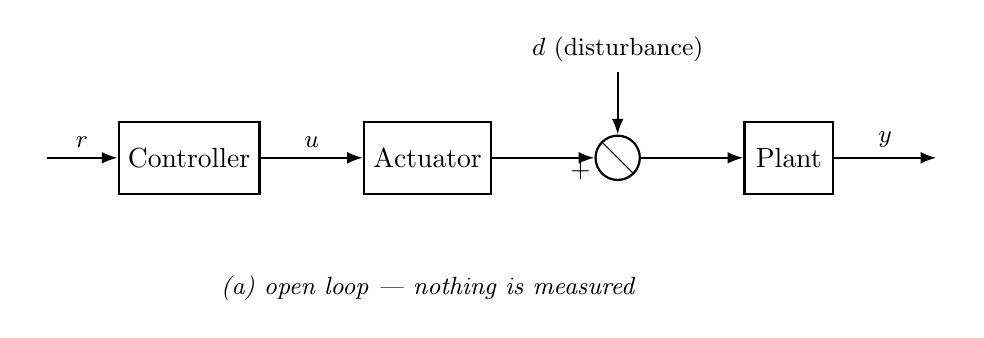
\begin{tikzpicture}[node distance=1.5cm and 1.3cm]
% ---- open loop ----
\node (r) at (0,0) {};
\node[block, right=0.9cm of r] (ctrl) {Controller};
\node[block, right=of ctrl] (act) {Actuator};
\node[sumnode, right=of act] (s1) {};
\node[block, right=of s1] (plant) {Plant};
\node[right=1.3cm of plant] (y) {};
\draw[sig] (r) -- node[above,font=\small]{$r$} (ctrl);
\draw[sig] (ctrl) -- node[above,font=\small]{$u$} (act);
\draw[sig] (act) -- (s1);
\draw[sig] (s1) -- (plant);
\draw[sig] (plant) -- node[above,font=\small]{$y$} (y);
\node[above=0.8cm of s1, font=\small] (d1) {$d$ (disturbance)};
\draw[sig] (d1) -- (s1);
\draw (s1.north west) -- (s1.south east);
\sumsign{s1}{200}{+}
\node[below=0.9cm of act, font=\small\itshape] {(a) open loop --- nothing is measured};
\end{tikzpicture}

\vspace{9mm}

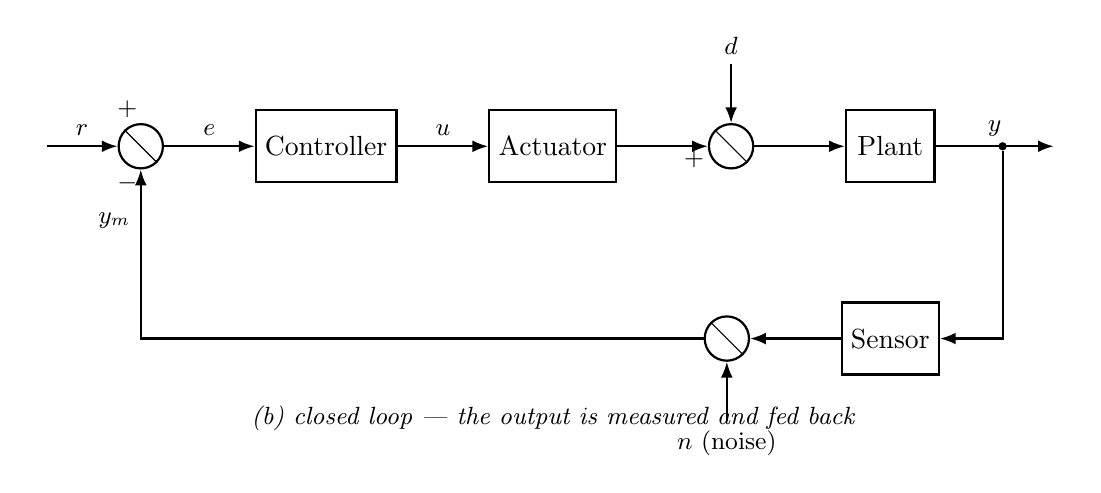
\begin{tikzpicture}[node distance=1.4cm and 1.15cm]
% ---- closed loop ----
\node (r) at (0,0) {};
\node[sumnode, right=0.9cm of r] (se) {};
\node[block, right=of se] (ctrl) {Controller};
\node[block, right=of ctrl] (act) {Actuator};
\node[sumnode, right=of act] (s1) {};
\node[block, right=of s1] (plant) {Plant};
\node[right=1.5cm of plant] (y) {};
\node[pickoff] at ($(plant.east)+(0.85,0)$) (po) {};
\node[block, below=1.5cm of plant] (sens) {Sensor};
\node[sumnode, left=of sens] (sn) {};

\draw[sig] (r) -- node[above,font=\small]{$r$} (se);
\draw[sig] (se) -- node[above,font=\small]{$e$} (ctrl);
\draw[sig] (ctrl) -- node[above,font=\small]{$u$} (act);
\draw[sig] (act) -- (s1);
\draw[sig] (s1) -- (plant);
\draw[sig] (plant) -- node[above,font=\small]{$y$} (y);
\node[above=0.75cm of s1, font=\small] (d1) {$d$};
\draw[sig] (d1) -- (s1);
\draw (s1.north west) -- (s1.south east);
\sumsign{s1}{200}{+}
\draw (se.north west) -- (se.south east);
\sumsign{se}{110}{+}
\sumsign{se}{250}{-}
\draw[sig] (po) |- (sens.east);
\draw[sig] (sens) -- (sn);
\node[below=0.75cm of sn, font=\small] (nn) {$n$ (noise)};
\draw[sig] (nn) -- (sn);
\draw (sn.north west) -- (sn.south east);
\draw[sig] (sn) -| node[pos=0.85,left,font=\small]{$y_m$} (se);
\node[below=2.7cm of act, font=\small\itshape] {(b) closed loop --- the output is measured and fed back};
\end{tikzpicture}
\caption{The two configurations. In (a) a disturbance $d$ passes straight
through to the output and is never corrected. In (b) its effect appears in the
measurement, hence in the error $e$, and the controller acts on it. The price
is the sensor, its cost, and its noise $n$. Cf.\ Nise Fig.~1.6, p.~8.}
\label{fig:openclosed}
\end{figure}

\begin{keyidea}
The distinguishing feature of an open-loop system is that it cannot compensate
for a disturbance. A closed-loop system corrects for disturbances \emph{it can
see in the measurement} --- and only for those.
\end{keyidea}

Nise's example is a toaster: its output is the colour of the toast, but it
measures time, not colour, so it cannot know that the bread is rye rather than
white, or thick rather than thin. Anyone who has burnt toast has performed the
experiment. A toaster \emph{oven} that measures reflectivity and humidity is
closed-loop --- and is several times the price. That trade-off is real and is
made on every project.

\subsection{Worked example: cruise control}

This example carries most of the intellectual content of the week. It is worth
following every line.

\begin{figure}[htbp]
\centering
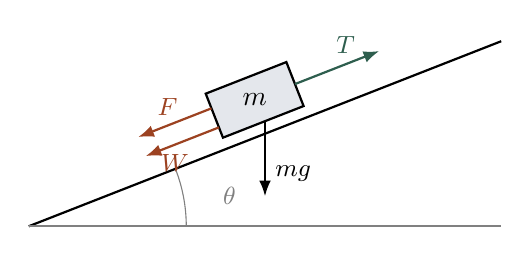
\begin{tikzpicture}[scale=1.0]
% road
\draw[thick] (-0.4,-0.25) -- (5.6,2.1);
\draw[thick,gray] (-0.4,-0.25) -- (5.6,-0.25);
\draw[gray] (1.6,-0.25) arc (0:21.4:2cm);
\node[gray,font=\small] at (2.15,0.13) {$\theta$};
% body
\begin{scope}[shift={(2.6,1.02)},rotate=21.4]
  \draw[thick,fill=fnavy!12] (-0.55,0.06) rectangle (0.55,0.66);
  \node at (0,0.36) {$m$};
  % thrust
  \draw[sig,faccent] (0.55,0.36) -- ++(1.15,0) node[above,pos=0.6,font=\small]{$T$};
  % friction + disturbance
  \draw[sig,fflag] (-0.55,0.46) -- ++(-1.0,0) node[above,pos=0.6,font=\small]{$F$};
  \draw[sig,fflag] (-0.55,0.2) -- ++(-1.0,0) node[below,pos=0.6,font=\small]{$W$};
\end{scope}
% weight
\draw[sig] (2.6,1.08) -- ++(0,-0.95) node[right,pos=0.7,font=\small]{$mg$};
\end{tikzpicture}
\caption{Forces on a vehicle on a road of slope $\theta$. Cf.\ Khalil
Fig.~1-1, p.~3.}
\label{fig:car}
\end{figure}

\begin{workedex}[title=Worked example 2.1 --- open- versus closed-loop cruise control]
\textbf{Model.} With $T=au$ the thrust from throttle angle $u$ and engine gain
$a$, $F=b\upsilon$ the road friction, and
$W=mg\sin\theta+D$ a disturbance made of the gradient term and aerodynamic
drag, Newton's second law along the road gives
\[
  m\dot{\upsilon}=T-F-W=au-b\upsilon-mg\sin\theta-D .
\]
Here $u$ is the control input, $\upsilon$ is the controlled output. Only the
engine gain $a$ is known reliably: the mass $m$ depends on how many passengers
are aboard, $b$ on the road surface, and $W$ on gradient and wind.

\medskip
\textbf{Open-loop design.} Design as if there were no disturbance, $W=0$, using
nominal values $\hat m$ and $\hat b$:
\[
  \hat m \dot\upsilon = au-\hat b \upsilon .
\]
At steady state $\dot\upsilon=0$, so $\upsilon_{ss}=au/\hat b$. To make
$\upsilon_{ss}$ equal the desired speed $\upsilon_{des}$, choose the constant
throttle
\[
  \boxed{\;u=\frac{\hat b\,\upsilon_{des}}{a}\;}
\]
Now apply that fixed $u$ to the \emph{real} car, which has the true $b$, the
true $m$, and a real disturbance $W$:
\[
  m\dot\upsilon = \hat b \upsilon_{des}-b\upsilon-W
  \quad\Longrightarrow\quad
  \upsilon_{ss}=\frac{\hat b\upsilon_{des}-W}{b},
\]
so the steady-state speed error is
\begin{equation}
  \upsilon_{des}-\upsilon_{ss}
  =\left(\frac{b-\hat b}{b}\right)\upsilon_{des}+\frac{1}{b}W .
  \label{eq:ol}
\end{equation}

\medskip
\textbf{Closed-loop design.} Measure $\upsilon$ with a speedometer and set
\begin{equation}
  u=\underbrace{\frac{\hat b\,\upsilon_{des}}{a}}_{\text{feedforward}}
   +\underbrace{K(\upsilon_{des}-\upsilon)}_{\text{feedback}} .
  \label{eq:cl-law}
\end{equation}
Substituting into the true model,
\[
  m\dot\upsilon=\hat b\upsilon_{des}+aK(\upsilon_{des}-\upsilon)-b\upsilon-W
   =-(b+aK)\upsilon+(\hat b+aK)\upsilon_{des}-W,
\]
and the steady-state error becomes
\begin{equation}
  \upsilon_{des}-\upsilon_{ss}
  =\left(\frac{b-\hat b}{b+aK}\right)\upsilon_{des}+\frac{1}{b+aK}W .
  \label{eq:cl}
\end{equation}

\medskip
\textbf{What it means.} Compare \eqref{eq:ol} and \eqref{eq:cl}. They are the
same expression with $b$ replaced by $b+aK$ in \emph{both} denominators. Making
the feedback gain $K$ large therefore shrinks \emph{both} error terms at once:
the term caused by not knowing $b$, and the term caused by the disturbance $W$.
One knob buys robustness to parameter error and rejection of disturbance
together. That is what feedback is for.
\end{workedex}

\begin{figure}[htbp]
\centering
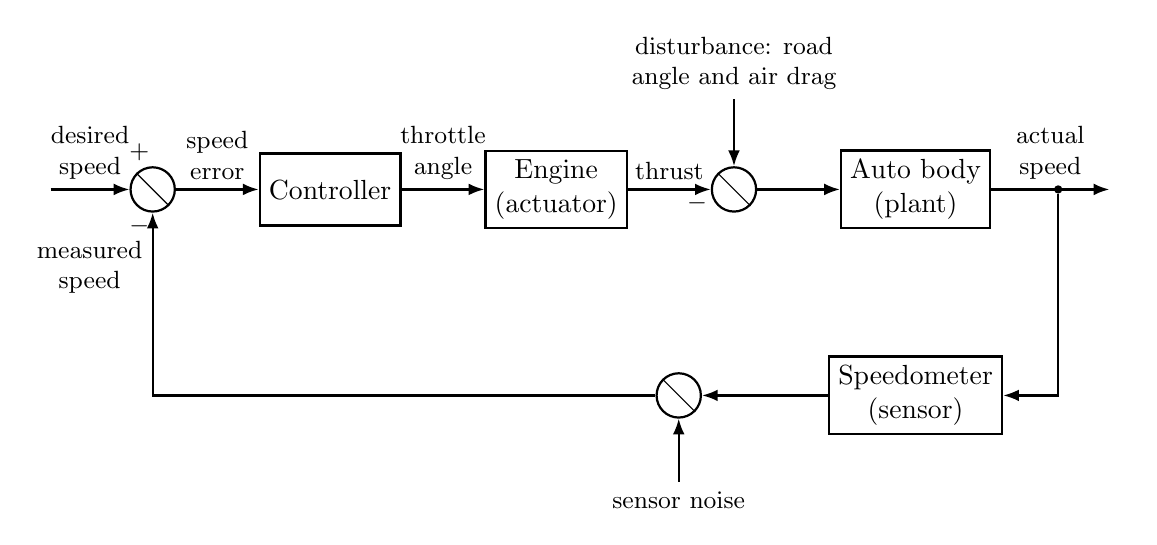
\begin{tikzpicture}[node distance=1.35cm and 1.05cm]
\node (r) at (0,0) {};
\node[sumnode, right=1.0cm of r] (se) {};
\node[block, right=of se] (ctrl) {Controller};
\node[block, right=of ctrl, align=center] (eng) {Engine\\(actuator)};
\node[sumnode, right=of eng] (s1) {};
\node[block, right=of s1, align=center] (body) {Auto body\\(plant)};
\node[right=1.5cm of body] (y) {};
\node[pickoff] at ($(body.east)+(0.85,0)$) (po) {};
\node[block, below=1.6cm of body, align=center] (sp) {Speedometer\\(sensor)};
\node[sumnode, left=1.6cm of sp] (sn) {};

\draw[sig] (r) -- node[above,align=center,font=\small]{desired\\speed} (se);
\draw[sig] (se) -- node[above,align=center,font=\small]{speed\\error} (ctrl);
\draw[sig] (ctrl) -- node[above,align=center,font=\small]{throttle\\angle} (eng);
\draw[sig] (eng) -- node[above,font=\small]{thrust} (s1);
\draw[sig] (s1) -- (body);
\draw[sig] (body) -- node[above,align=center,font=\small]{actual\\speed} (y);
\node[above=0.85cm of s1, align=center, font=\small] (d1)
   {disturbance: road\\angle and air drag};
\draw[sig] (d1) -- (s1);
\draw (s1.north west) -- (s1.south east);
\sumsign{s1}{200}{-}
\draw (se.north west) -- (se.south east);
\sumsign{se}{110}{+}
\sumsign{se}{250}{-}
\draw[sig] (po) |- (sp.east);
\draw[sig] (sp) -- (sn);
\node[below=0.8cm of sn, font=\small] (nn) {sensor noise};
\draw[sig] (nn) -- (sn);
\draw (sn.north west) -- (sn.south east);
\draw[sig] (sn) -| node[pos=0.85,left,align=center,font=\small]{measured\\speed} (se);
\end{tikzpicture}
\caption{The cruise-control loop of Worked example 2.1, showing the four basic
components: plant, actuator, sensor, controller. Cf.\ Khalil Fig.~1-2, p.~5.}
\label{fig:cruise}
\end{figure}

\subsection{Why not simply make $K$ enormous?}

Equation \eqref{eq:cl} suggests taking $K\to\infty$. Three things stop you, and
between them they account for most of the remaining eleven weeks
(Khalil, p.~5):

\begin{enumerate}[leftmargin=*]
\item \textbf{The actuator saturates.} A throttle angle has a maximum. Beyond
      it, extra commanded control does nothing. \emph{(Control constraints ---
      background only in this unit; examinable in FEE3412.)}
\item \textbf{Transient response degrades.} A large $K$ makes the response
      faster but more oscillatory, and the design specification usually limits
      overshoot. \emph{(Weeks 5, 8, 9.)}
\item \textbf{The system can become unstable.} Above some gain the closed loop
      no longer settles at all. This does not happen in the first-order cruise
      model above, but it is the norm once the plant has any real dynamics.
      \emph{(Weeks 7, 8, 10, 11, 12 --- this is the largest single theme of the
      unit.)}
\end{enumerate}

If you have ever heard a public-address system squeal when the volume is turned
up, you have heard instability caused by high-gain feedback.

\begin{pitfall}
Feedback is not free and it is not always better. It adds a sensor (cost,
noise, one more thing to fail) and it can destabilise a plant that was
perfectly well behaved open loop. ``Closed loop is better'' is not a theorem;
it is a trade-off, and the rest of this unit is the machinery for making the
trade deliberately.
\end{pitfall}

\subsection{Error versus actuating signal}

In Figure~\ref{fig:openclosed}(b) the signal leaving the first summing junction
is properly called the \emph{actuating signal}. It equals the true error
$r-y$ only when the input and output transducers both have gain~1. A
position loop whose feedback potentiometer produces \SI{0.5}{\volt\per\radian}
while the reference potentiometer produces \SI{1}{\volt\per\radian} has an
actuating signal that is \emph{not} proportional to $r-y$, and computing
steady-state error as though it were will give the wrong answer. We return to
this properly in Week~6 under \emph{non-unity feedback}.

% --------------------------------------------------------------------
\section{What a well-designed control system must do}
\label{sec:objectives}

Khalil (p.~6) lists six requirements. They are worth copying out, because they
are, almost exactly, the syllabus of this unit and the next.

\begin{center}
\begin{tabular}{@{}p{0.47\textwidth}p{0.47\textwidth}@{}}
\toprule
\textbf{Requirement} & \textbf{Where it is dealt with}\\
\midrule
The system must be \textbf{stable}: a well-behaved input must give a
well-behaved output. & Weeks 7 (Routh--Hurwitz), 8 (root locus),
11--12 (Nyquist). \\
The output must \textbf{track} the reference with zero or small
\textbf{steady-state error}. & Week 6 (static error constants, system type).\\
The \textbf{transient response} must be acceptable. & Weeks 5 (specifications),
8--9 (shaping it by gain).\\
The effect of \textbf{disturbance} and \textbf{measurement noise} should be
small. & Background reading only in FEE3411 (Khalil \S4-4 to \S4-8; Nise
\S7.5, \S7.7). Examinable in FEE3412.\\
The design must be \textbf{robust} to model uncertainty. & Introduced through
gain and phase margins, Weeks 10 and 12. Treated properly in FEE3412.\\
The design must respect \textbf{constraints} on the control input. &
Background only here; FEE3412.\\
\bottomrule
\end{tabular}
\end{center}

\begin{keyidea}
Stability, steady-state accuracy and transient response are the three things
FEE3411 teaches you to \emph{analyse}. FEE3412 teaches you to \emph{design} for
them. If you can say which of the three a question is about, you can usually
say which method it wants.
\end{keyidea}

\subsection{Where the mathematics comes from}

Every method in this unit needs a mathematical model of the plant. Models come
from (Khalil, p.~6):

\begin{itemize}[leftmargin=*]
\item \textbf{first principles} --- Kirchhoff's laws, Newton's laws, energy
      balances. This is Week~2.
\item \textbf{identification experiments} --- apply known inputs, measure the
      outputs, fit a model to the data. Outside this syllabus, but note that
      fitting a second-order model to a measured step response, which you do in
      the Week~5 tutorial, is identification in miniature.
\item \textbf{both} --- derive the structure from physics, then measure the
      parameters.
\end{itemize}

A model that captures everything is too complicated to design with. A model
that captures too little gives a design that fails on the real plant. Choosing
what to leave out is the hardest judgement in the subject and it requires
understanding the physics, not just the algebra.

\subsection{The design process as a map of the course}

Nise (\S1.5, p.~15, Fig.~1.11) sets out six steps. They are reproduced in
Figure~\ref{fig:design} with the week of this unit that covers each. Use it as
a map: when a topic feels disconnected, find it here.

\begin{figure}[htbp]
\centering
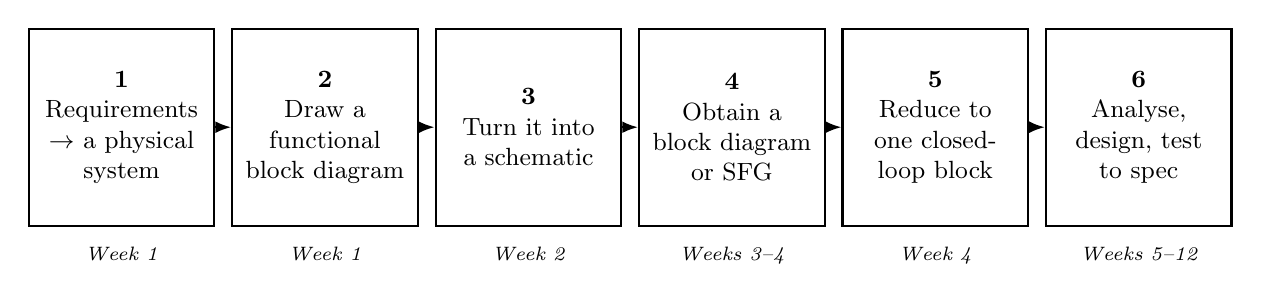
\begin{tikzpicture}[node distance=0.20cm,
  st/.style={draw, thick, rectangle, align=center, text width=2.18cm,
             minimum height=2.5cm, font=\small, inner sep=2.5pt}]
\node[st] (s1) {\textbf{1}\\Requirements\\$\rightarrow$ a physical system};
\node[st, right=of s1] (s2) {\textbf{2}\\Draw a functional block diagram};
\node[st, right=of s2] (s3) {\textbf{3}\\Turn it into a schematic};
\node[st, right=of s3] (s4) {\textbf{4}\\Obtain a block diagram or SFG};
\node[st, right=of s4] (s5) {\textbf{5}\\Reduce to one closed-loop block};
\node[st, right=of s5] (s6) {\textbf{6}\\Analyse, design, test to spec};
\foreach \a/\b in {s1/s2,s2/s3,s3/s4,s4/s5,s5/s6}
  \draw[sig] (\a) -- (\b);
\foreach \n/\w in {s1/{Week 1}, s2/{Week 1}, s3/{Week 2}, s4/{Weeks 3--4},
                   s5/{Week 4}, s6/{Weeks 5--12}}
  \node[below=0.14cm of \n, font=\scriptsize\itshape, text width=2.1cm,
        align=center] {\w};
\end{tikzpicture}
\caption{The design process; cf.\ Nise Fig.~1.11, p.~15, annotated with the
week of FEE3411 in which each step is taught. Steps 1 and 2 are this week.}
\label{fig:design}
\end{figure}

% --------------------------------------------------------------------
\section{The servomechanism}
\label{sec:servo}

\begin{keyidea}
A \textbf{servomechanism} (servo) is a feedback control system in which the
controlled variable is a mechanical position, or one of its derivatives
(velocity, acceleration).
\end{keyidea}

The servomechanism deserves its own name because it is the archetype: antenna
pointing, machine-tool slides, robot joints, radar dishes, aircraft control
surfaces, disc-drive head positioning, steering gear on ships. Almost every
worked example in this unit is, underneath, a servo.

Figure~\ref{fig:servo} shows the standard laboratory form. A pair of
potentiometers acts as the error detector: one is turned by the reference
shaft, the other by the load shaft, and both are fed from the same d.c.\
supply. The voltage between the two wipers is
\begin{equation}
  v_e = K_p\,(r-c),
  \label{eq:pot}
\end{equation}
where $r$ and $c$ are the reference and output shaft angles in radians and
$K_p$ is the potentiometer sensitivity in \si{\volt\per\radian}. The
subtraction is done by the wiring, not by a circuit: this is the physical
realisation of the summing junction drawn as $\otimes$ in
Figure~\ref{fig:openclosed}. The error voltage is amplified by $K_a$ and drives
the armature of a d.c.\ motor, which turns the load through a gear train of
ratio $n$ in the direction that reduces the error.

\begin{figure}[htbp]
\centering
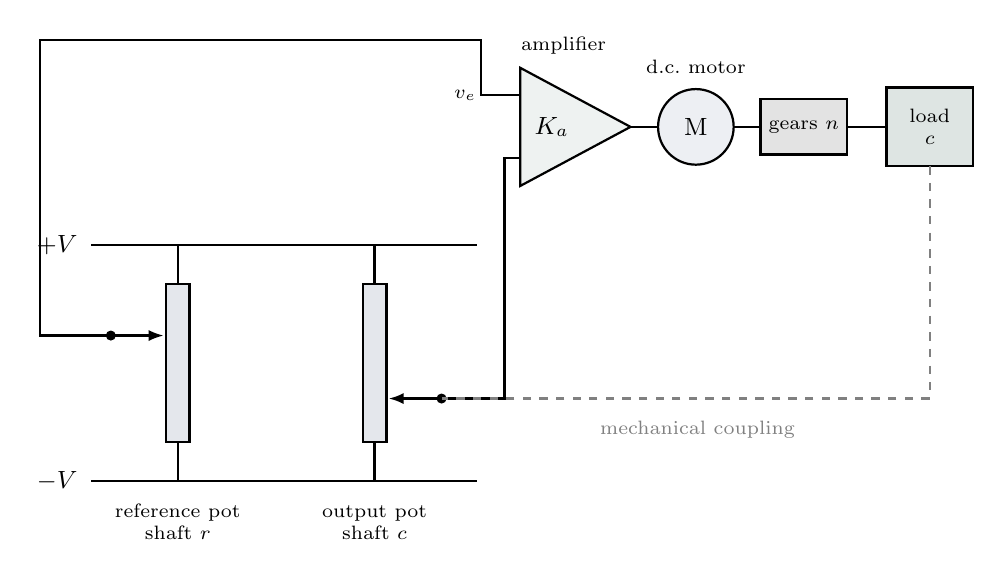
\begin{tikzpicture}[font=\small, x=1cm, y=1cm]
% ---- supply rails -------------------------------------------------
\draw[thick] (0.3,3.4) -- (5.2,3.4);
\draw[thick] (0.3,0.4) -- (5.2,0.4);
\node[left] at (0.25,3.4) {$+V$};
\node[left] at (0.25,0.4) {$-V$};
% ---- reference potentiometer --------------------------------------
\draw[thick] (1.4,3.4) -- (1.4,2.9);
\draw[thick] (1.4,0.9) -- (1.4,0.4);
\draw[thick,fill=fnavy!12] (1.25,0.9) rectangle (1.55,2.9);
\draw[thick,-{Latex[length=1.9mm]}] (0.55,2.25) -- (1.22,2.25);
\draw[fill] (0.55,2.25) circle (1.6pt);
\node[align=center,font=\scriptsize] at (1.4,-0.12) {reference pot\\shaft $r$};
% ---- output potentiometer -----------------------------------------
\draw[thick] (3.9,3.4) -- (3.9,2.9);
\draw[thick] (3.9,0.9) -- (3.9,0.4);
\draw[thick,fill=fnavy!12] (3.75,0.9) rectangle (4.05,2.9);
\draw[thick,-{Latex[length=1.9mm]}] (4.75,1.45) -- (4.08,1.45);
\draw[fill] (4.75,1.45) circle (1.6pt);
\node[align=center,font=\scriptsize] at (3.9,-0.12) {output pot\\shaft $c$};
% ---- leads from the two wipers to the amplifier --------------------
\draw[thick] (0.55,2.25) -- (-0.35,2.25) -- (-0.35,6.0) -- (5.25,6.0)
             -- (5.25,5.3) -- (5.75,5.3);
\draw[thick] (4.75,1.45) -- (5.55,1.45) -- (5.55,4.5) -- (5.75,4.5);
\node[font=\scriptsize] at (5.05,5.3) {$v_e$};
% ---- amplifier ----------------------------------------------------
\draw[thick,fill=faccent!8] (5.75,4.15) -- (5.75,5.65) -- (7.15,4.9) -- cycle;
\node at (6.15,4.9) {$K_a$};
\node[font=\scriptsize, above] at (6.3,5.7) {amplifier};
% ---- motor --------------------------------------------------------
\draw[thick] (7.15,4.9) -- (7.5,4.9);
\draw[thick,fill=fnavy!8] (7.98,4.9) circle (0.48);
\node at (7.98,4.9) {M};
\node[font=\scriptsize, above] at (7.98,5.45) {d.c.\ motor};
% ---- gear train ---------------------------------------------------
\draw[thick] (8.46,4.9) -- (8.8,4.9);
\draw[thick,fill=gray!22] (8.8,4.55) rectangle (9.9,5.25);
\node[font=\scriptsize] at (9.35,4.9) {gears $n$};
% ---- load ---------------------------------------------------------
\draw[thick] (9.9,4.9) -- (10.4,4.9);
\draw[thick,fill=faccent!16] (10.4,4.4) rectangle (11.5,5.4);
\node[font=\scriptsize,align=center] at (10.95,4.9) {load\\$c$};
% ---- mechanical coupling back to the output pot --------------------
\draw[thick,dashed,gray] (10.95,4.4) -- (10.95,1.45) -- (4.75,1.45);
\node[gray,font=\scriptsize,align=center] at (8.0,1.05)
      {mechanical coupling};
\end{tikzpicture}
\caption{Position servomechanism with a potentiometer-pair error detector. The
two wipers are the summing junction: the voltage between them is
$K_p(r-c)$. Cf.\ Nagrath \& Gopal (2nd ed.) \S5.4, p.~137, whose Fig.~5.6 (p.~138) is this
schematic with its block diagram; we derive that block diagram in Week~4 and
its response in Week~5.}
\label{fig:servo}
\end{figure}

\paragraph{Regulator or tracking system?} Two duties are worth distinguishing,
because they lead to different specifications:
\begin{itemize}[leftmargin=*]
\item a \textbf{regulator} holds the output at a constant reference in the face
      of disturbances --- speed governor, voltage regulator, temperature
      control;
\item a \textbf{tracking (follow-up) system} makes the output follow a
      reference that is itself changing --- a radar dish following an aircraft,
      a machine-tool axis following a profile.
\end{itemize}
The same hardware often does both. The distinction matters in Week~6, where the
steady-state error depends on whether the reference is a step, a ramp or a
parabola.

% ====================================================================
\part*{Part B --- Control system components and devices}
\addcontentsline{toc}{part}{Part B}

\noindent
This half of the lecture is a \emph{survey}. The syllabus outcome is ELO~1,
``describe the working principles'', and that is the depth expected: you should
be able to say what a device does, how it does it, and roughly what its
transfer function looks like. Deriving those transfer functions is Week~2 and,
in more detail, FEE3412, which contains a full hardware block.

\begin{figure}[htbp]
\centering
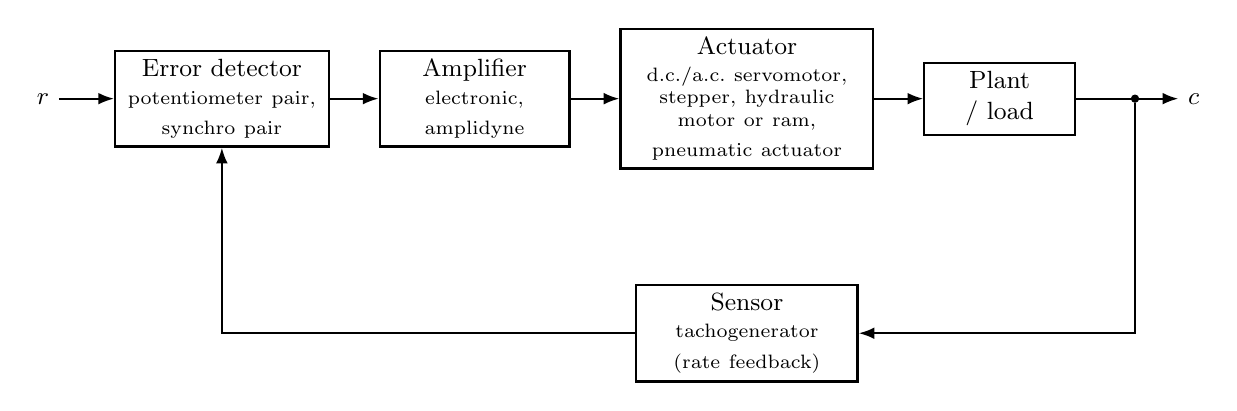
\begin{tikzpicture}[node distance=0.62cm, font=\small,
   bb/.style={block, align=center, inner sep=3pt}]
\node[bb, text width=2.5cm] (ed)
  {Error detector\\[2pt]{\scriptsize potentiometer pair,\\ synchro pair}};
\node[bb, right=of ed, text width=2.2cm] (am)
  {Amplifier\\[2pt]{\scriptsize electronic,\\ amplidyne}};
\node[bb, right=of am, text width=3.0cm] (ac)
  {Actuator\\[2pt]{\scriptsize d.c./a.c.\ servomotor,\\ stepper, hydraulic\\
   motor or ram,\\ pneumatic actuator}};
\node[bb, right=of ac, text width=1.7cm] (pl) {Plant\\/ load};
\node[bb, below=1.45cm of ac, text width=2.6cm] (se)
  {Sensor\\[2pt]{\scriptsize tachogenerator\\ (rate feedback)}};
\node[left=0.7cm of ed] (rr) {$r$};
\node[right=1.3cm of pl] (cc) {$c$};
\node[pickoff] at ($(pl.east)+(0.75,0)$) (po) {};
\draw[sig] (rr) -- (ed);
\draw[sig] (ed) -- (am);
\draw[sig] (am) -- (ac);
\draw[sig] (ac) -- (pl);
\draw[sig] (pl) -- (cc);
\draw[sig] (po) |- (se.east);
\draw[sig] (se) -| (ed);
\end{tikzpicture}
\caption{Where each family of components sits in the loop. Everything in
Part~B is one of these four boxes.}
\label{fig:chain}
\end{figure}

% --------------------------------------------------------------------
\section{Error detectors}

The error detector performs the subtraction $r-c$ physically. Two standard
devices do it for angular position.

\subsection{The potentiometer pair}

Described in \S\ref{sec:servo} and Figure~\ref{fig:servo}. Its virtues are that
it is cheap, it is a d.c.\ device (the output is a d.c.\ voltage proportional
to the error), and its model, equation~\eqref{eq:pot}, is a pure gain $K_p$
with no dynamics. Its vices are wiper friction, finite resolution set by the
winding pitch, wear, and electrical noise from the sliding contact.

\subsection{The synchro pair}

For anything that must run continuously, or turn through many revolutions, or
survive a hostile environment, the sliding contact is unacceptable. The
\emph{synchro} (trade names \emph{selsyn}, \emph{autosyn}) replaces it with
transformer action. Nagrath \S4.3, p.~92.

A \textbf{synchro transmitter} is built like a small three-phase alternator. The
stator carries three identical Y-connected coils with their axes
\SI{120}{\degree} apart; the rotor carries a single concentric coil fed with
a.c.\ through slip rings. Applying $v(t)=V_r\sin\omega_c t$ to the rotor sets up
a sinusoidally distributed air-gap flux along the rotor axis. By transformer
action a voltage is induced in each stator coil, proportional to the cosine of
the angle between that coil's axis and the rotor axis. With the rotor at angle
$\theta$ from the axis of coil $S_2$, the coil-to-neutral voltages are
\[
  v_{s_1n}=KV_r\sin\omega_c t\,\cos(\theta+120^\circ),\quad
  v_{s_2n}=KV_r\sin\omega_c t\,\cos\theta,\quad
  v_{s_3n}=KV_r\sin\omega_c t\,\cos(\theta+240^\circ).
\]

\begin{keyidea}
The synchro transmitter is a single-phase transformer whose rotor coil is the
primary and whose three stator coils are the secondaries. Its input is a shaft
angle; its output is three a.c.\ voltages whose magnitudes encode that angle.
\end{keyidea}

The three stator terminals are wired to the stator of a \textbf{synchro control
transformer}, which is built the same way except that its rotor is cylindrical,
so the air gap --- and hence the rotor output impedance --- does not change as
it turns. Circulating currents reproduce in the control transformer's air gap
the same flux pattern the transmitter had, so the voltage induced in the
control transformer rotor is proportional to the cosine of the angle between
the two rotors:
\[
  e(t)=K'V_r\cos\phi\,\sin\omega_c t .
\]
With the rotors displaced by $\theta$ and $\alpha$ from their respective
electrical zeros, $\phi=90^\circ-\theta+\alpha$ and
\begin{equation}
  e(t)=K'V_r\sin(\theta-\alpha)\sin\omega_c t
      \;\approx\; K_s(\theta-\alpha)\sin\omega_c t
      \quad\text{for small }(\theta-\alpha),
  \label{eq:synchro}
\end{equation}
where $K_s$ is the \textbf{sensitivity of the error detector} in
\si{\volt\per\radian} (rms per radian of shaft difference).

\begin{figure}[htbp]
\centering
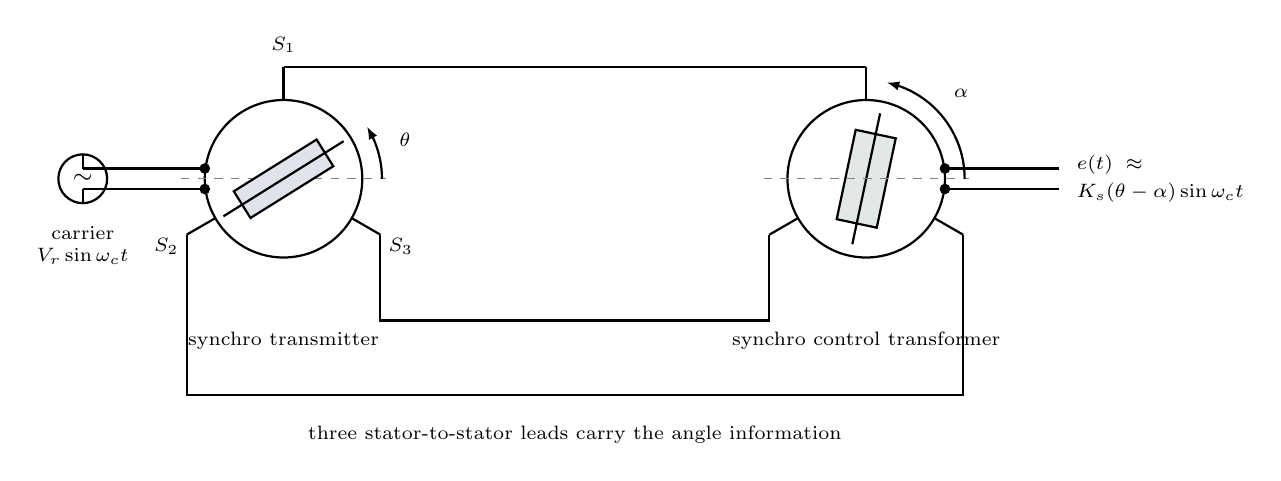
\begin{tikzpicture}[font=\small, x=1cm, y=1cm]
\def\R{1.0}\def\S{1.42}
% ================= transmitter =================
\draw[thick] (0,0) circle (\R);
\foreach \a in {90,210,330}{\draw[thick] (\a:\R) -- (\a:\S);}
\node[font=\scriptsize] at (90:{\S+0.28}) {$S_1$};
\node[font=\scriptsize] at (210:{\S+0.30}) {$S_2$};
\node[font=\scriptsize] at (330:{\S+0.30}) {$S_3$};
% rotor (single coil) at angle theta
\draw[dashed,gray] (-1.3,0) -- (1.3,0);
\begin{scope}[rotate=32]
  \draw[thick,fill=fnavy!14] (-0.62,-0.20) rectangle (0.62,0.20);
  \draw[thick] (-0.9,0) -- (0.9,0);
\end{scope}
\draw[thick,-{Latex[length=1.6mm]}] (1.25,0) arc (0:32:1.25);
\node[font=\scriptsize] at (18:1.62) {$\theta$};
\node[font=\scriptsize] at (0,-2.05) {synchro transmitter};
% slip rings and carrier supply (rotor leads out to the left)
\draw[fill] (-1.0,0.13) circle (1.7pt);
\draw[fill] (-1.0,-0.13) circle (1.7pt);
\draw[thick] (-1.0,0.13) -- (-2.55,0.13);
\draw[thick] (-1.0,-0.13) -- (-2.55,-0.13);
\draw[thick] (-2.55,0.13) -- (-2.55,0.30);
\draw[thick] (-2.55,-0.13) -- (-2.55,-0.30);
\draw[thick] (-2.55,0.30) circle (0) ;
\node[draw,thick,circle,minimum size=0.62cm] at (-2.55,0) {};
\node at (-2.55,0) {$\sim$};
\node[font=\scriptsize,align=center] at (-2.55,-0.85) {carrier\\$V_r\sin\omega_c t$};
% ================= control transformer =================
\begin{scope}[shift={(7.4,0)}]
\draw[thick] (0,0) circle (\R);
\foreach \a in {90,210,330}{\draw[thick] (\a:\R) -- (\a:\S);}
\begin{scope}[rotate=78]
  \draw[thick,fill=faccent!14] (-0.58,-0.26) rectangle (0.58,0.26);
  \draw[thick] (-0.85,0) -- (0.85,0);
\end{scope}
\draw[dashed,gray] (-1.3,0) -- (1.3,0);
\draw[thick,-{Latex[length=1.6mm]}] (1.25,0) arc (0:78:1.25);
\node[font=\scriptsize] at (42:1.62) {$\alpha$};
\node[font=\scriptsize] at (0,-2.05) {synchro control transformer};
% rotor output
\draw[fill] (1.0,0.13) circle (1.7pt);
\draw[fill] (1.0,-0.13) circle (1.7pt);
\draw[thick] (1.0,0.13) -- (2.45,0.13);
\draw[thick] (1.0,-0.13) -- (2.45,-0.13);
\node[font=\scriptsize,align=left,anchor=west] at (2.55,0)
   {$e(t)\;\approx$\\[2pt] $K_s(\theta-\alpha)\sin\omega_c t$};
\end{scope}
% ================= the three stator leads =================
\draw[thick] (0,\S) -- (7.4,\S);
\draw[thick] (-1.23,-0.71) -- (-1.23,-2.75) -- (8.63,-2.75) -- (8.63,-0.71);
\draw[thick] (1.23,-0.71) -- (1.23,-1.80) -- (6.17,-1.80) -- (6.17,-0.71);
\node[font=\scriptsize, align=center] at (3.7,-3.25)
   {three stator-to-stator leads carry the angle information};
\end{tikzpicture}
\caption{Synchro transmitter and control transformer used as an error detector.
Cf.\ Nagrath \& Gopal Fig.~4.12, p.~94. The three
stator-to-stator leads carry the angle information; there is no sliding contact
in the signal path.}
\label{fig:synchro}
\end{figure}

The output in \eqref{eq:synchro} is a carrier $\sin\omega_c t$ whose
\emph{amplitude} carries the error, and whose \emph{phase reverses} when the
error changes sign. This is \textbf{suppressed-carrier modulation}. A control
system whose internal signals are of this form is called a \textbf{carrier
control system}, and it is analysed on the basis of the modulating signal
alone, which is valid provided the signal bandwidth is much lower than the
carrier frequency.

\begin{pitfall}
In a carrier system the useful information is the \emph{envelope}, not the
instantaneous value. A student who tries to read the error off an oscilloscope
trace of $e(t)$ directly, instead of its envelope, will conclude the error is
oscillating at \SI{400}{\hertz} when the shaft is standing still.
\end{pitfall}

% --------------------------------------------------------------------
\section{Electric actuators}

\subsection{The d.c.\ servomotor}

The workhorse. A d.c.\ motor becomes a servomotor when it is built for low
inertia and rapid reversal. Two ways of controlling it:

\begin{itemize}[leftmargin=*]
\item \textbf{Armature control} --- field current held constant, armature
      voltage varied. The one used almost universally, and the one whose
      transfer function we derive from first principles in the Week~2 tutorial.
\item \textbf{Field control} --- armature current held constant, field voltage
      varied. Cheaper amplifier (the field carries less current) but slower,
      because the field circuit has a large inductance.
\end{itemize}

The armature-controlled motor driving inertia $J$ and viscous friction $f$ has
the transfer function
\begin{equation}
  \frac{\theta_m(s)}{V_a(s)}=\frac{K_m}{s(\tau_m s+1)} .
  \label{eq:dcm}
\end{equation}
Note the shape --- an integrator in series with a first-order lag. Keep it in
mind; \S\ref{sec:shape} is about why it keeps recurring.

Large d.c.\ systems historically used an \textbf{amplidyne} --- a rotating
power amplifier. It is a cross-field d.c.\ machine carrying two brush sets
\SI{90}{\degree} apart; the quadrature-axis brushes are short-circuited through
a series quadrature winding, so the machine delivers two stages of power
amplification in one frame (Nagrath \S4.3, p.~90). It has been displaced by
thyristor and IGBT drives, but it appears in older textbook problems and you
should recognise the name.

\subsection{The a.c.\ (two-phase) servomotor}

Preferred at low power, and where a synchro error detector already makes the
signals a.c.\ It is rugged, light, and has no brushes. Nagrath \S4.3, p.~84.

Structurally it is a two-phase induction motor: two stator windings
\SI{90}{\degree} apart in space, excited by voltages \SI{90}{\degree} apart in
time. That produces a rotating field of constant magnitude; the field induces
currents in the short-circuited rotor and the interaction produces torque in
the direction of field rotation. Two design changes make it a servomotor:

\begin{enumerate}[leftmargin=*]
\item \textbf{High rotor resistance}, so that the ratio $X/R$ is small. In an
      ordinary induction motor $X/R$ is deliberately large, which puts maximum
      torque near the operating point and makes the torque--speed curve highly
      nonlinear --- and, over part of its range, \emph{positively} sloped. A
      positive slope means negative effective damping, which can make the
      closed loop unstable. This is precisely why an ordinary induction motor
      cannot be used as a servomotor.
\item \textbf{Unbalanced excitation.} One winding, the \emph{reference phase},
      is fed with a fixed voltage. The other, the \emph{control phase}, is fed
      from the servo amplifier with a variable-magnitude voltage at
      $\pm\SI{90}{\degree}$ to the reference. Reversing the sign of the control
      voltage reverses the direction of rotation. The rotor is a small-diameter
      squirrel cage or a drag cup, to keep inertia low.
\end{enumerate}

\begin{figure}[htbp]
\centering
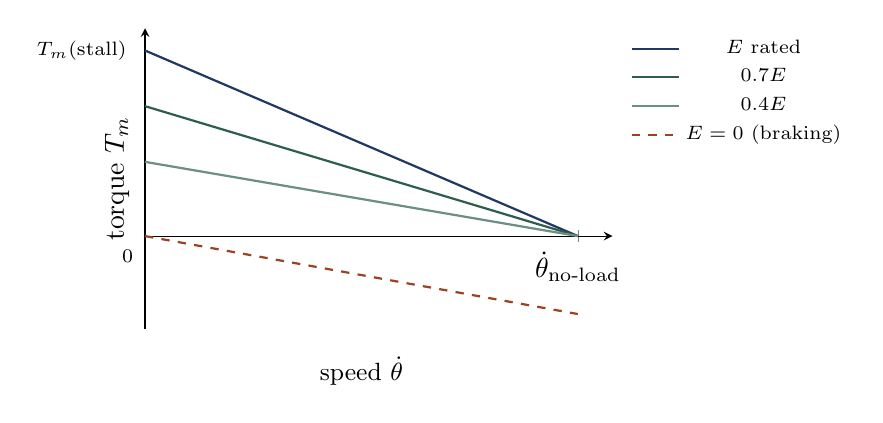
\begin{tikzpicture}
\begin{axis}[width=0.62\textwidth, height=5.4cm,
  ylabel={torque $T_m$},
  xmin=0, xmax=1.08, ymin=-0.5, ymax=1.12,
  xtick={0,1}, xticklabels={$0$,$\dot\theta_{\text{no-load}}$},
  ytick=\empty, axis y line=left, axis x line=middle, clip=false,
  legend style={font=\scriptsize, draw=none, at={(1.02,1.0)}, anchor=north west}]
\addplot[fnavy, thick, domain=0:1, samples=2]{1-x};
\addlegendentry{$E$ rated}
\addplot[faccent, thick, domain=0:1, samples=2]{0.7*(1-x)};
\addlegendentry{$0.7E$}
\addplot[faccent!70, thick, domain=0:1, samples=2]{0.4*(1-x)};
\addlegendentry{$0.4E$}
\addplot[fflag, thick, dashed, domain=0:1, samples=2]{-0.42*x};
\addlegendentry{$E=0$ (braking)}
\node[font=\scriptsize, anchor=east] at (axis cs:-0.02,1.0) {$T_m$(stall)};
\node[font=\scriptsize, anchor=north east] at (axis cs:-0.005,-0.02) {$0$};
\node[font=\small, anchor=north] at (axis cs:0.5,-0.60) {speed $\dot\theta$};
\end{axis}
\end{tikzpicture}
\caption{Torque--speed characteristics of a two-phase servomotor at several
control-phase voltages, idealised as the straight lines used for linearisation.
All slopes are negative --- that is the whole point of the high-resistance
rotor. At zero control voltage the motor develops a \emph{decelerating} torque,
so that line passes through the origin with negative slope. Cf.\ Nagrath \&
Gopal Fig.~4.6, p.~86.}
\label{fig:acservo}
\end{figure}

Torque depends on both speed and control voltage, $T_m=f(\dot\theta,E)$. Expanding
in a Taylor series about an operating point and keeping first-order terms
(the linearisation technique of Week~2),
\[
  \Delta T_m = K\,\Delta E - f\,\Delta\dot\theta,
  \qquad
  K=\left.\frac{\partial T_m}{\partial E}\right|_0,\quad
  f=-\left.\frac{\partial T_m}{\partial \dot\theta}\right|_0 .
\]
With a load of inertia $J$ and friction $f_0$, $\;\Delta T_m=J\Delta\ddot\theta
+f_0\Delta\dot\theta$, and taking Laplace transforms,
\begin{equation}
  G_m(s)=\frac{\Delta\theta(s)}{\Delta E(s)}
        =\frac{K}{Js^2+(f_0+f)s}
        =\frac{K_m}{s(\tau_m s+1)},
  \qquad K_m=\frac{K}{f_0+f},\quad \tau_m=\frac{J}{f_0+f}.
  \label{eq:acm}
\end{equation}

\begin{keyidea}
The negative slope of the torque--speed characteristic acts as extra viscous
friction $f$, added to the load's own $f_0$. If the slope were positive,
$f_0+f$ could go negative --- negative damping --- and the system would be
unstable. Stability considerations reach right down into the choice of rotor
resistance.
\end{keyidea}

The two constants are obtained from two standard tests: the \textbf{stall
torque} test (rotor held, rated control voltage) and the \textbf{no-load speed}
test. The straight line joining those two points is the working approximation
to the characteristic, so
\[
  K\approx\frac{\text{stall torque at rated voltage}}
                {\text{rated control-phase voltage}},
  \qquad
  f\approx\frac{\text{stall torque at rated voltage}}
                {\text{no-load speed at rated voltage}} .
\]
Nagrath notes (\S4.3, eq.~4.7, p.~88) that in real servomotors the slope at low
speed is nearer \emph{half} the slope at rated voltage, so for position control
work $f$ is often taken as half the value above.

\subsection{The stepper motor}

A \textbf{stepper motor} converts a train of input pulses into a train of
discrete angular steps, one step per pulse. It is the actuator of incremental
motion control: printers, tape and capstan drives, machine tools, plotters,
3-D printers. Nagrath \S4.4, p.~99.

The common types are \emph{variable reluctance} and \emph{permanent magnet}. In
a variable-reluctance stepper the stator stacks are pulse-excited and the
rotors are unexcited; both are toothed. When a stator stack is energised the
rotor is pulled to the nearest \textbf{minimum-reluctance} position, where the
teeth line up. That aligned position is stable; the position where rotor teeth
face stator slots is unstable.

While the teeth on all rotors are aligned with each other, the stator teeth of
successive stacks are offset by
\begin{equation}
  \alpha=\frac{360^\circ}{n\,T},
  \label{eq:step}
\end{equation}
where $n$ is the number of stacks (equal to the number of phases) and $T$ the
number of rotor teeth. That angle $\alpha$ is the \textbf{step angle}. For
$n=3$ stacks and $T=12$ teeth, $\alpha=\SI{10}{\degree}$. Exciting the phases
in the order $abcabc\ldots$ steps the rotor one way; $bacbac\ldots$ steps it
the other. \emph{Directional control requires three or more phases} --- with
two, the sequence is the same read forwards or backwards.

\begin{figure}[htbp]
\centering
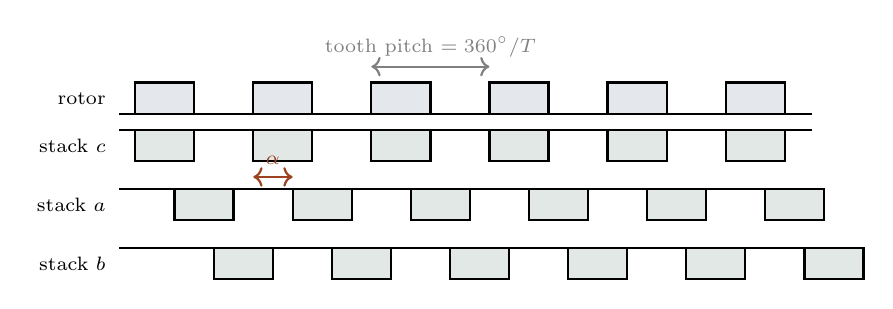
\begin{tikzpicture}[font=\small, scale=1.0]
% rotor teeth (aligned across all stacks)
\foreach \i in {0,...,5}{
  \draw[thick,fill=fnavy!12] ({\i*1.5},2.35) rectangle ({\i*1.5+0.75},2.75);}
\draw[thick] (-0.2,2.35) -- (8.6,2.35);
\node[left, font=\scriptsize] at (-0.25,2.55) {rotor};
% stack c : aligned
\foreach \i in {0,...,5}{
  \draw[thick,fill=faccent!14] ({\i*1.5},1.75) rectangle ({\i*1.5+0.75},2.15);}
\draw[thick] (-0.2,2.15) -- (8.6,2.15);
\node[left, font=\scriptsize] at (-0.25,1.95) {stack $c$};
% stack a : offset by alpha
\foreach \i in {0,...,5}{
  \draw[thick,fill=faccent!14] ({\i*1.5+0.5},1.0) rectangle ({\i*1.5+1.25},1.4);}
\draw[thick] (-0.2,1.4) -- (8.6,1.4);
\node[left, font=\scriptsize] at (-0.25,1.2) {stack $a$};
% stack b : offset by 2 alpha
\foreach \i in {0,...,5}{
  \draw[thick,fill=faccent!14] ({\i*1.5+1.0},0.25) rectangle ({\i*1.5+1.75},0.65);}
\draw[thick] (-0.2,0.65) -- (8.6,0.65);
\node[left, font=\scriptsize] at (-0.25,0.45) {stack $b$};
% dimension for alpha
\draw[<->, thick, fflag] (1.5,1.55) -- (2.0,1.55);
\node[fflag, font=\scriptsize, above] at (1.75,1.58) {$\alpha$};
% tooth pitch
\draw[<->, thick, gray] (3.0,2.95) -- (4.5,2.95);
\node[gray, font=\scriptsize, above] at (3.75,2.95) {tooth pitch $=360^\circ/T$};
\end{tikzpicture}
\caption{Developed (rolled-out) view of a three-stack variable-reluctance
stepper. Rotor teeth are aligned across all stacks; stator stacks are offset
successively by $\alpha=360^\circ/nT$. Energising $c$, then $a$, then $b$ pulls
the rotor one step $\alpha$ at a time. Cf.\ Nagrath \& Gopal Figs.~4.18 and
4.20, pp.~100--101.}
\label{fig:stepper}
\end{figure}

Two consequences matter for control:

\begin{itemize}[leftmargin=*]
\item \textbf{The stepper is a digital actuator}, so shaft position is
      determined entirely by the pulse count. An \emph{open-loop} step servo
      can therefore reach the accuracy of a closed-loop analogue system, with
      no position sensor at all. This is the rare case where open loop is the
      right engineering answer.
\item \textbf{The price of that is skipped steps.} If pulses arrive faster than
      the rotor can settle, or if the rotor oscillates too much about the lock
      position, a step is lost --- and, since nothing is measured, lost
      silently and permanently. High-performance systems therefore close the
      loop after all, gating the pulse train from a position feedback signal.
\end{itemize}

The dynamic model is genuinely nonlinear. With inductance varying
cosinusoidally with rotor angle, $L(\theta)=L_1+L_2\cos T\theta$, the reluctance
torque is
\[
  T_m=\tfrac{1}{2}i^2\frac{\partial L}{\partial\theta}=-K\,i^2(t)\sin T\theta ,
\]
which no linear approximation captures usefully. Stepper dynamics are solved
numerically, not analytically --- one reason steppers do not appear in the
analysis weeks of this unit.

% --------------------------------------------------------------------
\section{Sensors: the tachogenerator}

A \textbf{tachogenerator} (tachometer) produces a voltage proportional to shaft
speed:
\begin{equation}
  v_t = K_t\,\dot\theta ,\qquad [K_t]=\si{\volt\per\radian\per\second}.
  \label{eq:tacho}
\end{equation}

\begin{itemize}[leftmargin=*]
\item A \textbf{d.c.\ tachogenerator} is a small permanent-magnet d.c.\
      generator. Output polarity follows the direction of rotation. Ripple from
      commutation is its main limitation.
\item An \textbf{a.c.\ (drag-cup) tachogenerator} has two stator coils in space
      quadrature and a thin aluminium cup for a rotor, rotating in the air gap
      of a fixed magnetic structure (Nagrath \S4.3, p.~88). The reference coil
      is excited; rotation induces speed voltages in the cup, whose currents
      set up a quadrature flux, and the emf induced in the quadrature coil is
      proportional to speed. The very low rotor inertia is its advantage.
\end{itemize}

Tachogenerators are used in two distinct ways, and it is worth separating them
now:

\begin{enumerate}[leftmargin=*]
\item as the \textbf{sensor of a speed control loop}, where speed is the
      controlled variable;
\item as \textbf{rate feedback} inside a \emph{position} loop, where the
      tachometer signal is subtracted in an inner loop to add damping.
\end{enumerate}

The second is the more interesting. Nagrath's a.c.\ position control system
(\S4.3, p.~96; Fig.~4.14, p.~97) uses a synchro pair, an a.c.\ amplifier, an a.c.\
servomotor, gearing, \emph{and} an a.c.\ tachometer for rate feedback, giving
the closed-loop transfer function
\[
  \frac{\theta_c(s)}{\theta_r(s)}
   =\frac{K_mK_aK_s\,n}{\tau_m s^2+(1+K_mK_aK_t)s+K_mK_aK_s n},
\]
in which the tachometer constant $K_t$ appears only in the $s$ coefficient ---
the damping term. Adding rate feedback improves damping without changing the
steady-state gain. That is your first sight of a compensator, and it is the
reason to notice it now: we will meet it as a design tool in Week~9 and study
it properly in FEE3412.

% --------------------------------------------------------------------
\section{Hydraulic power elements}

Where the load is large, hydraulics win. A hydraulic motor is far smaller than
an electric motor of the same power output, and hydraulic components are fast
and rugged. Against that: leaks, sealing against contamination, noise, and
sluggishness at low temperature as the oil thickens; and hydraulic lines are
not as flexible as cables. Typical uses are power steering and brakes, ship
steering gear, large machine tools, aircraft flight controls, and excavators.
Nagrath \S4.5, p.~104.

Hydraulic output devices split by the motion they produce:
\begin{itemize}[leftmargin=*]
\item \textbf{rotary output} --- \emph{hydraulic motors} (this is what the
      syllabus phrase ``rotary actuators'' refers to);
\item \textbf{translational output} --- \emph{hydraulic linear actuators}, i.e.\
      cylinders and rams.
\end{itemize}

\subsection{Pump--motor transmission}

The classical arrangement is a \textbf{variable-stroke pump} driving a
\textbf{fixed-stroke motor}. Both are axial-piston machines: pistons in a
rotating cylinder block bear on a wobble (swash) plate. With the wobble plate
in the neutral position the pistons do not reciprocate and no oil is pumped.
Tilt the plate through the \emph{stroke angle} $x$ and each piston strokes once
per revolution, delivering oil at a rate proportional to $x$. Reversing the
tilt reverses the flow, and hence reverses the motor. Control is exercised by
one mechanical variable: the stroke angle.

The model follows from a flow balance and a torque balance:
\[
\begin{aligned}
  q_p &= K_p x &&\text{(ideal pump flow, proportional to stroke angle)}\\
  q_m &= K_m\dot\theta &&\text{(motor flow, proportional to motor speed)}\\
  q_\ell &= K_\ell p &&\text{(leakage, proportional to pressure drop)}\\
  q_c &= K_c\,\dot p &&\text{(compressibility flow)}\\
  q_p &= q_m+q_\ell+q_c &&\text{(continuity)}\\
  T_m &= K_T p = J\ddot\theta+f\dot\theta &&\text{(torque balance at the load)}
\end{aligned}
\]
Eliminating $p$ and neglecting compressibility ($K_c\ll K_m$) gives
\begin{equation}
  G(s)=\frac{\theta(s)}{X(s)}=\frac{K}{s(\tau s+1)} .
  \label{eq:hyd}
\end{equation}
The same shape as \eqref{eq:dcm} and \eqref{eq:acm}.

\subsection{Valve control}

Instead of varying the pump stroke, hold the supply pressure constant and
throttle the flow with a \textbf{spool valve}. The moving part of a valve is
far lighter than a pump's stroke mechanism, so the time constants are much
smaller and the system is much faster. The cost is that valve flow is
genuinely nonlinear: flow through a sharp-edged orifice goes as
$\sqrt{\Delta p}$, so the linear model
\begin{equation}
  q = K_1 x - K_2 p
  \label{eq:valve}
\end{equation}
is a linearisation valid only for small spool displacements about neutral.
(Week~2 shows the technique that produces $K_1$ and $K_2$.)

A \textbf{three-way} valve has supply, sump and one service port; a
\textbf{four-way} valve has two service ports and can drive a double-acting
cylinder in both directions, which is what Figure~\ref{fig:spool} shows. When
the spool is at neutral, $x=0$, all flow is blocked. Move it one way and the
supply is connected to one side of the piston while the other side drains to
sump; move it the other way and the connections swap.

\begin{figure}[htbp]
\centering
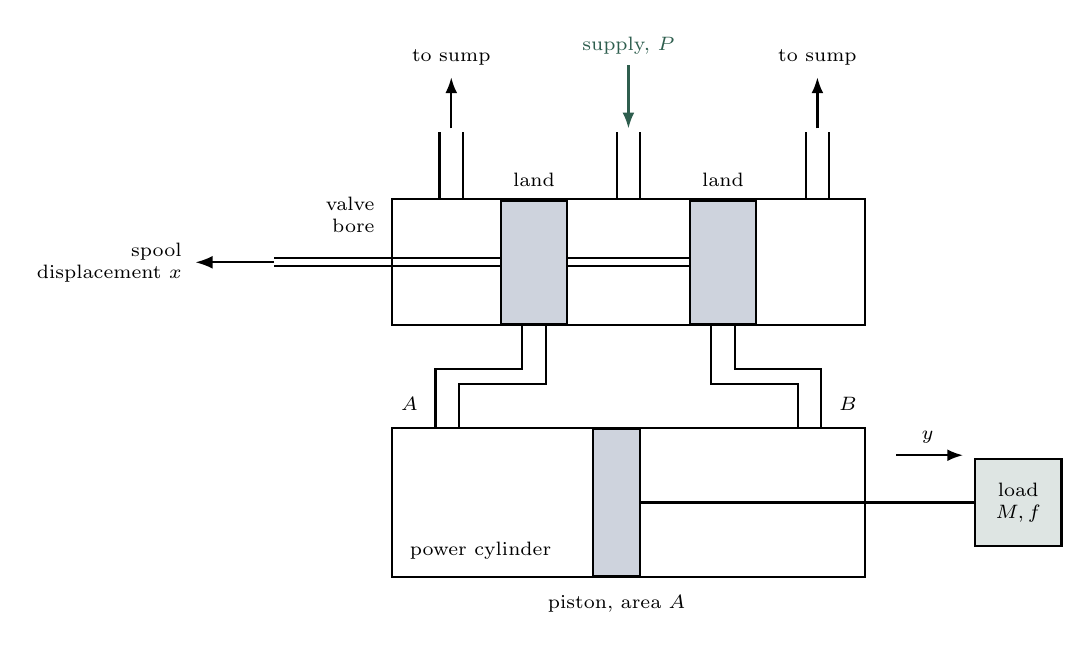
\begin{tikzpicture}[font=\small, x=1cm, y=1cm]
% ---------------- valve body (bore) ----------------
\draw[thick] (0.6,4.6) rectangle (6.6,6.2);
\node[font=\scriptsize, left, align=right] at (0.5,6.0) {valve\\bore};
% ---------------- spool: stem + two lands ----------------
\draw[thick] (-0.9,5.35) -- (2.4,5.35);
\draw[thick] (-0.9,5.45) -- (2.4,5.45);
\draw[thick] (2.4,5.35) -- (4.8,5.35);
\draw[thick] (2.4,5.45) -- (4.8,5.45);
\foreach \c in {2.4,4.8}{
  \draw[thick,fill=fnavy!22] (\c-0.42,4.62) rectangle (\c+0.42,6.18);}
\node[font=\scriptsize, above] at (2.4,6.24) {land};
\node[font=\scriptsize, above] at (4.8,6.24) {land};
\draw[thick,-{Latex[length=2.2mm]}] (-0.9,5.4) -- (-1.9,5.4);
\node[font=\scriptsize, left, align=right] at (-1.95,5.4)
      {spool\\displacement $x$};
% ---------------- ports on the top face ----------------
% supply, centre
\draw[thick] (3.45,6.2) -- (3.45,7.05);
\draw[thick] (3.75,6.2) -- (3.75,7.05);
\draw[sig, faccent] (3.6,7.9) -- (3.6,7.1);
\node[faccent, font=\scriptsize, above, align=center] at (3.6,7.92)
      {supply, $P$};
% two sump returns, outer
\foreach \c in {1.35,6.0}{
  \draw[thick] (\c-0.15,6.2) -- (\c-0.15,7.05);
  \draw[thick] (\c+0.15,6.2) -- (\c+0.15,7.05);
  \draw[sig] (\c,7.1) -- (\c,7.75);
  \node[font=\scriptsize, above] at (\c,7.78) {to sump};}
% ---------------- service ports on the bottom face ----------------
\draw[thick] (2.25,4.6) -- (2.25,4.05) -- (1.15,4.05) -- (1.15,3.3);
\draw[thick] (2.55,4.6) -- (2.55,3.85) -- (1.45,3.85) -- (1.45,3.3);
\node[font=\scriptsize, left] at (1.05,3.6) {$A$};
\draw[thick] (4.65,4.6) -- (4.65,3.85) -- (5.75,3.85) -- (5.75,3.3);
\draw[thick] (4.95,4.6) -- (4.95,4.05) -- (6.05,4.05) -- (6.05,3.3);
\node[font=\scriptsize, right] at (6.15,3.6) {$B$};
% ---------------- power cylinder ----------------
\draw[thick] (0.6,1.4) rectangle (6.6,3.3);
\draw[thick,fill=fnavy!22] (3.15,1.42) rectangle (3.75,3.28);
\node[font=\scriptsize, below] at (3.45,1.3) {piston, area $A$};
\node[font=\scriptsize, above right] at (0.7,1.5) {power cylinder};
% rod and load
\draw[very thick] (3.75,2.35) -- (8.0,2.35);
\draw[thick,fill=faccent!16] (8.0,1.8) rectangle (9.1,2.9);
\node[font=\scriptsize, align=center] at (8.55,2.35) {load\\$M,f$};
\draw[sig] (7.0,2.95) -- (7.85,2.95);
\node[font=\scriptsize, above] at (7.4,2.98) {$y$};
\end{tikzpicture}
\caption{Four-way spool valve controlling a double-acting power cylinder --- a
hydraulic linear actuator. Spool displacement $x$ admits high-pressure oil to
one side of the piston and vents the other to sump; the differential pressure
drives the load a distance $y$. Cf.\ Nagrath \& Gopal Fig.~4.27, p.~111
(the section begins on p.~110).}
\label{fig:spool}
\end{figure}

\subsection{The linear actuator (cylinder)}

Take Figure~\ref{fig:spool} and write down three equations. The linearised
valve relation \eqref{eq:valve}; continuity, with flow into the cylinder equal
to swept volume rate, $q=A\dot y$; and the force balance on the load, driven by
the differential pressure acting on the piston area $A$:
\[
  Ap = M\ddot y + f\dot y .
\]
Eliminating $q$ and $p$:
\begin{equation}
  \frac{Y(s)}{X(s)}=\frac{K}{s(\tau s+1)},
  \qquad K=\frac{K_1}{A},\qquad \tau=\frac{MK_2}{A^2+K_2 f}\;\;\text{(approx.)}
  \label{eq:cyl}
\end{equation}
Again the same shape.

\begin{pitfall}
Note where the $1/s$ comes from. It is \emph{not} an approximation and it is
not the motor's inertia. Flow into a cylinder sets the piston's \emph{velocity},
so position is the integral of the input. Any actuator whose input commands a
rate --- valve opening $\to$ velocity, armature voltage $\to$ speed, pump stroke
$\to$ motor speed --- carries a free integrator when the output of interest is
position. Recognising this saves you an algebra step in half the problems in
this course.
\end{pitfall}

% --------------------------------------------------------------------
\section{Pneumatic power elements}
\label{sec:pneu}

Pneumatic systems use air rather than oil. Air is non-inflammable, has
negligible viscosity, and does not change viscosity with temperature the way
hydraulic oil does. But air is compressible, so pneumatic systems have
substantial compressibility flow and are characterised by \textbf{longer time
delays} --- the reason they dominate in \emph{process} control, where plants are
slow anyway, and are rare where speed matters. Nagrath \S4.6, p.~116.

\subsection{Bellows}

A hollow chamber with thin corrugated side walls and flat end faces. It behaves
as a spring. Separating force $=(\Delta P)A$; restoring force $=K(\Delta x)$;
so at equilibrium
\begin{equation}
  \frac{\Delta X(s)}{\Delta P(s)}=\frac{A}{K}.
  \label{eq:bellows}
\end{equation}
A pure gain: pressure in, displacement out.

\subsection{The flapper--nozzle valve}

The key pneumatic sensing element. Air at constant supply pressure $P_s$ passes
through a fixed \emph{orifice} and out of a \emph{nozzle}. A pivoted
\emph{flapper} sits in front of the nozzle at distance $e$. Move the flapper
closer and the restriction increases, so the nozzle back pressure $P_b$ rises
towards $P_s$; move it away and $P_b$ falls towards ambient.

\begin{figure}[htbp]
\centering
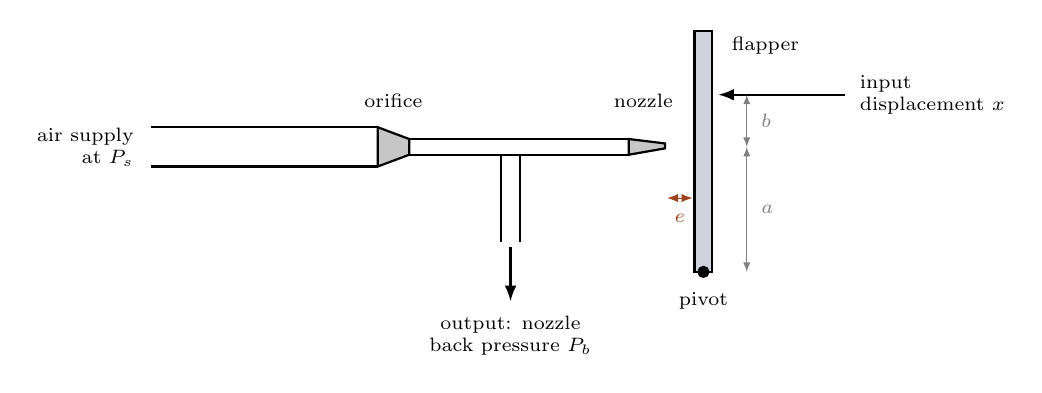
\begin{tikzpicture}[font=\small, x=1.25cm, y=1.25cm]
% ---- supply line and fixed orifice ----
\draw[thick] (0,1.62) -- (2.3,1.62);
\draw[thick] (0,2.02) -- (2.3,2.02);
\node[font=\scriptsize, left, align=right] at (-0.08,1.82)
      {air supply\\at $P_s$};
\draw[thick,fill=gray!45] (2.3,2.02) -- (2.62,1.90) -- (2.62,1.74)
                          -- (2.3,1.62) -- cycle;
\node[font=\scriptsize, above] at (2.46,2.12) {orifice};
% ---- chamber up to the nozzle ----
\draw[thick] (2.62,1.90) -- (4.85,1.90);
\draw[thick] (2.62,1.74) -- (4.85,1.74);
% ---- back-pressure tap ----
\draw[thick] (3.55,1.74) -- (3.55,0.85);
\draw[thick] (3.75,1.74) -- (3.75,0.85);
\draw[sig] (3.65,0.80) -- (3.65,0.25);
\node[font=\scriptsize, below, align=center] at (3.65,0.20)
      {output: nozzle\\back pressure $P_b$};
% ---- nozzle ----
\draw[thick,fill=gray!45] (4.85,1.90) -- (5.22,1.855) -- (5.22,1.805)
                          -- (4.85,1.74) -- cycle;
\node[font=\scriptsize, above] at (5.0,2.12) {nozzle};
% ---- flapper on a pivot ----
\draw[thick,fill=fnavy!22] (5.52,0.55) rectangle (5.70,3.00);
\node[font=\scriptsize, right] at (5.80,2.85) {flapper};
\draw[fill] (5.61,0.55) circle (2pt);
\node[font=\scriptsize, below] at (5.61,0.44) {pivot};
% ---- the gap e ----
\draw[{Latex[length=1.4mm]}-{Latex[length=1.4mm]}, fflag]
      (5.24,1.30) -- (5.50,1.30);
\node[fflag, font=\scriptsize, below] at (5.37,1.24) {$e$};
% ---- input displacement ----
\draw[sig] (7.05,2.35) -- (5.76,2.35);
\node[font=\scriptsize, right, align=left] at (7.10,2.35)
      {input\\displacement $x$};
% ---- lever arms ----
\draw[{Latex[length=1.2mm]}-{Latex[length=1.2mm]}, gray]
      (6.05,0.55) -- (6.05,1.82);
\node[gray, font=\scriptsize, right] at (6.10,1.19) {$a$};
\draw[{Latex[length=1.2mm]}-{Latex[length=1.2mm]}, gray]
      (6.05,1.82) -- (6.05,2.35);
\node[gray, font=\scriptsize, right] at (6.10,2.09) {$b$};
\end{tikzpicture}
\caption{Flapper--nozzle valve. Small movements of the flapper produce large
changes in back pressure --- a high-gain displacement-to-pressure transducer.
Cf.\ Nagrath \& Gopal Fig.~4.34, p.~117.}
\label{fig:flapper}
\end{figure}

The characteristic $P_b$ against $e$ is nonlinear, but has a steep linear
region which is the operating region. There,
\begin{equation}
  \frac{\Delta P_b(s)}{\Delta X(s)}=\left(\frac{a}{a+b}\right)K,
  \qquad K<0,
  \label{eq:flapper}
\end{equation}
where $a$ and $b$ are the lever arms from the pivot to the nozzle and to the
input point, so that $e=[a/(a+b)]x$. The gain is negative: closer flapper,
higher pressure.

\subsection{The pneumatic relay}

Keeping the flapper motion small enough to stay linear keeps the output
pressure swing small too, so a pneumatic power amplifier --- a \textbf{relay}
--- is put in cascade. A ball on the lower bellows surface seats either on its
upper seat (closing the vent, so output pressure rises to supply) or on its
lower seat (shutting off supply, so output falls to ambient). Moving the
flapper \emph{away} from the nozzle drops $P_b$, the bellows contracts, the
ball moves up, the vent closes and the output pressure \emph{rises}. The relay
therefore inverts the sign as well as amplifying:
\begin{equation}
  \frac{\Delta P(s)}{\Delta X(s)}=\left(\frac{a}{a+b}\right)K,\qquad K>0 .
  \label{eq:relay}
\end{equation}

\subsection{The pneumatic (diaphragm) actuator}

Most pneumatic control systems need translational output. A diaphragm of area
$A$ is exposed to the controlled pressure and moves a stem against a spring of
stiffness $K$, with the load contributing mass $M$ and friction $f$:
\[
  A\,\Delta P = M\Delta\ddot y+f\Delta\dot y+K\Delta y
\]
\begin{equation}
  \Longrightarrow\quad
  \frac{\Delta Y(s)}{\Delta P(s)}=\frac{A}{Ms^2+fs+K}.
  \label{eq:pneuact}
\end{equation}

\begin{figure}[htbp]
\centering
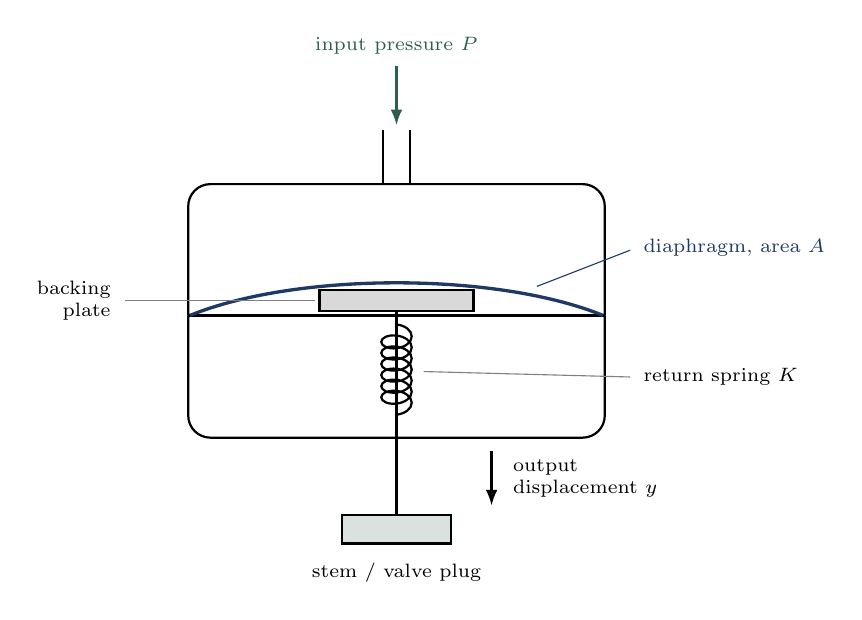
\begin{tikzpicture}[font=\small, x=1.15cm, y=1.15cm]
% ---- housing ----
\draw[thick, rounded corners=8pt] (0.7,2.30) -- (0.7,3.75) -- (5.3,3.75)
                                  -- (5.3,2.30);
\draw[thick, rounded corners=8pt] (0.7,2.30) -- (0.7,0.95) -- (5.3,0.95)
                                  -- (5.3,2.30);
\draw[thick] (0.7,2.30) -- (5.3,2.30);
% ---- diaphragm ----
\draw[very thick, fnavy] (0.72,2.30) .. controls (1.9,2.78) and (4.1,2.78)
                         .. (5.28,2.30);
\node[fnavy, font=\scriptsize, anchor=west] at (5.62,3.05)
     {diaphragm, area $A$};
\draw[fnavy] (5.58,3.02) -- (4.55,2.62);
% ---- pressure inlet ----
\draw[thick] (2.85,3.75) -- (2.85,4.35);
\draw[thick] (3.15,3.75) -- (3.15,4.35);
\draw[sig, faccent] (3.0,5.05) -- (3.0,4.40);
\node[faccent, font=\scriptsize, above] at (3.0,5.08) {input pressure $P$};
% ---- backing plate ----
\draw[thick,fill=gray!30] (2.15,2.35) rectangle (3.85,2.58);
\node[font=\scriptsize, anchor=east, align=right] at (-0.05,2.46)
     {backing\\plate};
\draw[gray] (0.0,2.46) -- (2.10,2.46);
% ---- stem ----
\draw[very thick] (3.0,2.35) -- (3.0,0.10);
% ---- return spring ----
\draw[thick, decorate, decoration={coil, aspect=0.6, segment length=4pt,
      amplitude=5.5pt}] (3.0,2.20) -- (3.0,1.15);
\node[font=\scriptsize, anchor=west] at (5.62,1.62) {return spring $K$};
\draw[gray] (5.58,1.62) -- (3.30,1.68);
% ---- output ----
\draw[sig] (4.05,0.80) -- (4.05,0.20);
\node[font=\scriptsize, anchor=west, align=left] at (4.18,0.50)
     {output\\displacement $y$};
\draw[thick,fill=faccent!18] (2.40,-0.22) rectangle (3.60,0.10);
\node[font=\scriptsize, below] at (3.0,-0.33) {stem / valve plug};
\end{tikzpicture}
\caption{Pneumatic diaphragm actuator. Unlike the hydraulic cylinder, the spring
gives it a definite equilibrium position for each pressure --- so its transfer
function \eqref{eq:pneuact} is second order with \emph{no} free integrator.
Cf.\ Nagrath \& Gopal Fig.~4.37, p.~119.}
\label{fig:pneuact}
\end{figure}

\begin{pitfall}
Compare \eqref{eq:pneuact} with \eqref{eq:cyl}. The hydraulic cylinder has a
free $1/s$; the spring-loaded pneumatic actuator does not. The difference is
the spring: with a spring present, a constant pressure gives a constant
\emph{position}; without one, a constant flow gives a constant \emph{velocity}.
Read the physics, not the picture.
\end{pitfall}

\subsection{Comparison}

\begin{center}
\begin{tabular}{@{}p{0.185\textwidth}p{0.245\textwidth}p{0.245\textwidth}p{0.245\textwidth}@{}}
\toprule
 & \textbf{Electric} & \textbf{Hydraulic} & \textbf{Pneumatic}\\
\midrule
Working medium & electric current & incompressible oil & compressible air\\
Power/weight & moderate & very high & low\\
Speed of response & fast & fastest under load & slow (compressibility)\\
Stiffness under load & moderate & very high & low\\
Typical use & instruments, servos, drives & machine tools, steering, aircraft
controls, presses & process control valves\\
Main drawback & limited torque density & leaks, sealing, contamination, noise &
long time delays, low stiffness\\
Safety & sparks & fire risk from oil mist & non-inflammable, intrinsically
safe\\
\bottomrule
\end{tabular}
\end{center}

% --------------------------------------------------------------------
\section{The shape that keeps recurring}
\label{sec:shape}

Collect the transfer functions from Part~B:

\begin{center}
\begin{tabular}{@{}llc@{}}
\toprule
\textbf{Device} & \textbf{Transfer function} & \textbf{Equation}\\
\midrule
Armature-controlled d.c.\ motor & $\theta/V_a = K_m/[s(\tau_m s+1)]$ & \eqref{eq:dcm}\\
Two-phase a.c.\ servomotor & $\theta/E = K_m/[s(\tau_m s+1)]$ & \eqref{eq:acm}\\
Hydraulic pump--motor transmission & $\theta/X = K/[s(\tau s+1)]$ & \eqref{eq:hyd}\\
Hydraulic linear actuator & $Y/X = K/[s(\tau s+1)]$ & \eqref{eq:cyl}\\
\addlinespace
Potentiometer error detector & $V_e/(r-c)=K_p$ & \eqref{eq:pot}\\
Synchro error detector & $E/(\theta-\alpha)=K_s$ & \eqref{eq:synchro}\\
Tachogenerator & $V_t/\dot\theta = K_t$ & \eqref{eq:tacho}\\
Pneumatic bellows & $\Delta X/\Delta P = A/K$ & \eqref{eq:bellows}\\
\addlinespace
Pneumatic diaphragm actuator & $\Delta Y/\Delta P = A/(Ms^2+fs+K)$ & \eqref{eq:pneuact}\\
\bottomrule
\end{tabular}
\end{center}

\begin{keyidea}
Almost every \emph{positional actuator} in control engineering, whatever its
physics, has the transfer function
\[
  G(s)=\frac{K}{s(\tau s+1)} .
\]
The $1/s$ is there because the input commands a rate and the output of interest
is the integral of that rate. The $1/(\tau s+1)$ is there because inertia and
friction resist that rate. Sensors and error detectors, by contrast, are
usually pure gains.
\end{keyidea}

This is not a coincidence to be noted and forgotten. It is why the same handful
of standard forms carry the whole unit:
\begin{itemize}[leftmargin=*]
\item Put $K/[s(\tau s+1)]$ in a unity-feedback loop and you get a
      \emph{second-order system} --- Week~5, and its $\zeta$ and $\omega_n$.
\item The free integrator makes the open loop \emph{type~1}, so it tracks a
      step with zero steady-state error and a ramp with a finite one --- Week~6.
\item Its pole--zero pattern (one pole at the origin, one on the negative real
      axis) gives the most common root locus you will ever sketch --- Week~8.
\item Its Bode plot is the sum of a $-\SI{20}{\decibel/decade}$ line and one
      corner --- Week~10.
\end{itemize}

% --------------------------------------------------------------------
\section*{Summary}

\begin{itemize}[leftmargin=*]
\item A control system makes a variable behave in a desired way without
      continuous human intervention. Its parts are plant, actuator, sensor,
      controller; its signals are reference, control input, disturbance,
      controlled output and measurement noise.
\item Open-loop control applies a precomputed input and measures nothing;
      closed-loop control measures the output and corrects. Only closed-loop
      control can reject a disturbance.
\item In the cruise-control example, feedback with gain $K$ replaces $b$ by
      $b+aK$ in the steady-state error, reducing both the parameter-error term
      and the disturbance term. See \eqref{eq:ol} and \eqref{eq:cl}.
\item Gain cannot be raised without limit: actuators saturate, transient
      response degrades, and the loop may become unstable.
\item A servomechanism is a feedback system whose controlled variable is
      mechanical position or a derivative of it.
\item Error detectors: potentiometer pair (d.c., gain $K_p$, sliding contact)
      and synchro pair (a.c., gain $K_s$, no sliding contact, suppressed-carrier
      output).
\item Actuators: d.c.\ servomotor (armature or field control), two-phase a.c.\
      servomotor (high rotor resistance for a negatively sloped, near-linear
      torque--speed curve), stepper motor (digital, step angle $360^\circ/nT$,
      usable open loop but can skip steps), hydraulic pump--motor and
      valve-plus-cylinder, pneumatic diaphragm actuator.
\item Sensors: tachogenerator, $v_t=K_t\dot\theta$, used both as the sensor of a
      speed loop and as rate feedback to add damping to a position loop.
\item Hydraulics give high power density and stiffness; pneumatics are safe and
      cheap but slow because air is compressible.
\item Positional actuators almost universally have the form $K/[s(\tau s+1)]$;
      error detectors and sensors are usually pure gains.
\end{itemize}

% --------------------------------------------------------------------
\section*{Before the tutorial}

These are not the tutorial sheet. They are the minimum you should be able to do
before you walk in. The tutorial hour itself is a review of the mathematical
toolkit --- Laplace transform pairs and properties, partial fractions, complex
numbers and the $s$-plane, and the standard test signals --- so revise
Khalil Appendix~A (p.~438) or Nise \S2.2 (p.~35) beforehand.

\begin{enumerate}[leftmargin=*]
\item A domestic pressure cooker holds pressure with a weighted valve that
      lifts when the internal pressure exceeds a set value. Is this open-loop
      or closed-loop? Identify the plant, the controlled variable, the sensor,
      the actuator and the reference. What is the disturbance?

\item In Worked example 2.1, suppose the engine gain is
      $a=\SI{20}{\newton\per\degree}$, the true friction coefficient is
      $b=\SI{50}{\newton\second\per\metre}$ while the nominal value used in
      design was $\hat b=\SI{45}{\newton\second\per\metre}$, the disturbance is
      $W=\SI{200}{\newton}$ and the desired speed is
      $\upsilon_{des}=\SI{25}{\metre\per\second}$. Compute the steady-state
      speed error open loop from \eqref{eq:ol}, and closed loop from
      \eqref{eq:cl} with $K=10$. By what factor does feedback improve it?

\item A three-stack variable-reluctance stepper motor has 20 rotor teeth. What
      is its step angle? How many pulses are needed for one full revolution of
      the rotor? If the load must be positioned to \SI{0.5}{\degree}, is this
      motor adequate on its own, and if not, name two ways to fix it.

\item Write down, without deriving them, the transfer function of (a) an
      armature-controlled d.c.\ servomotor driving an inertial load, (b) a
      hydraulic valve-and-cylinder actuator, and (c) a spring-loaded pneumatic
      diaphragm actuator. Which one is the odd one out, and why?

\item Sketch, from memory, the block diagram of Figure~\ref{fig:openclosed}(b),
      labelling every signal and every block. You will draw this diagram more
      times in the next eleven weeks than any other.
\end{enumerate}

% --------------------------------------------------------------------
\section*{Looking ahead}

This week gave you the vocabulary and the hardware. Everything after it is
mathematics applied to that vocabulary. \textbf{Week~2} derives models from
first principles --- electrical networks, translational and rotational
mechanical systems --- and in the tutorial builds the armature-controlled d.c.\
servomotor driving a load through a gear train, which is the transfer function
\eqref{eq:dcm} quoted here without proof. It also covers linear approximation
to nonlinear systems, the technique used informally in \S6 to linearise the
a.c.\ servomotor's torque--speed surface and the spool valve's orifice flow.
\textbf{Week~3} converts those models into transfer functions and moves into
the $s$-plane; \textbf{Week~4} connects them into block diagrams and reduces
them.

Two boundaries worth stating explicitly now. First, \emph{components are survey
depth in FEE3411}. You need to describe working principles (ELO~1); you are not
expected to design a servomotor or select a valve. FEE3412 contains a full
hardware block and treats these devices properly. Second, \emph{FEE3411 owns
analysis and FEE3412 owns design}. We will learn to predict what a system does
and to say whether it is stable, accurate and fast enough. Choosing a
compensator to \emph{make} it stable, accurate and fast --- lead, lag,
lag-lead, PID synthesis --- belongs to FEE3412. The one exception is a single
hour in Week~9 on design specifications and gain adjustment, which is
orientation, not synthesis. When you meet the phrase ``design a compensator''
in Khalil Ch.~5 or Nise Ch.~9 and 11, treat it as a forward reference: worth
reading, not examinable here.

Finally, note that the disturbance $d$ and noise $n$ drawn in
Figure~\ref{fig:openclosed}(b) will mostly be set to zero for the rest of this
unit. They are drawn because they are physically always present, and because
their rejection is one of the six objectives in \S\ref{sec:objectives}. Their
quantitative treatment (Khalil \S4-4 to \S4-8; Nise \S7.5, \S7.7) is background
reading here and examinable in FEE3412.

\end{document}
